\documentclass[11pt]{article}
\usepackage[a4paper,left=2.4cm,right=2.4cm,top=2.2cm,bottom=2.3cm]{geometry}
\usepackage[T1]{fontenc}
\usepackage{charter}
\usepackage[scaled=0.9]{helvet}
\usepackage{microtype}
\usepackage{graphicx}
\usepackage{booktabs}
\usepackage{float}
\usepackage{array}
\usepackage[hang,flushmargin]{footmisc}
\usepackage{enumitem}
\usepackage{titlesec}
\usepackage[hidelinks,pdftitle={Price and basket, more than foot traffic},pdfauthor={Bruno Fajardo Rosati},pdfsubject={Revenue drivers across 27 brands at one Delhi market},pdfkeywords={variance decomposition, extensive margin, intensive margin, price discrimination}]{hyperref}
\urlstyle{same}
\linespread{1.06}
\setlength{\parindent}{0pt}
\setlength{\parskip}{5.5pt}
\titleformat{\section}{\normalfont\bfseries}{\thesection\quad}{0pt}{}
\titlespacing*{\section}{0pt}{11pt}{2pt}
\renewcommand{\footnoterule}{\vspace*{-3pt}\noindent\rule{0.25\textwidth}{0.4pt}\vspace*{2.6pt}}
\setlength{\footnotesep}{9pt}
\pagestyle{plain}
\newcommand{\figtitle}[2]{\par\noindent{\bfseries #1}\par\vspace{1pt}\noindent{\small #2}\par\vspace{5pt}}
\newcommand{\fignote}[1]{\par\vspace{3pt}\noindent{\footnotesize\raggedright #1\par}}
\newcommand{\INR}{INR\,}
\newcommand{\x}{$\times$}
\begin{document}

{\LARGE\bfseries Price and basket, more than foot traffic\par}
\vspace{4pt}
{\large What explains revenue differences across 27 brands at one Delhi market\par}
\vspace{8pt}
Bruno Fajardo Rosati\footnote{brunofajardorosati@gmail.com. Data and code: \href{https://github.com/brunorosati/delhi-market-basket}{github.com/brunorosati/delhi-market-basket}.}\quad October 2026

\vspace{4pt}
{\small\textbf{Abstract.} On 12 April 2026, 27 brands sold at a market in Vasant Kunj, New Delhi, organized by TETR College of Business. I split each brand's revenue into its number of customers, units per customer and price per unit. Across brands, price per unit accounts for about half of the variance in log revenue and customer count for about a quarter. Montrega, the fragrance brand I co-founded, ranked first with the median number of customers and 6.1 bottles per customer, four times its basket at the other market it won. A single customer who bought more than ten bottles leaves most of that gap in place. With 27 brands and one evening of trading, the results describe one market and identify no cause.\par}

\section{Data}
The organizer published a leaderboard at 22:00 listing each brand's unique customers, units sold and revenue in Indian rupees (INR). I transcribed all 27 rows and checked each one against the leaderboard. The printed total (534 customers, 1,067 units, \INR516,029) is the sum of ranks 1 to 26 and leaves out Bumba, ranked 27th; with Bumba the market totals 553 customers, 1,089 units and \INR519,979. Every result below uses all 27 brands. For comparison I use the leaderboard of a second TETR market, Galleria Market (18 brands, 21:00; the leaderboard prints no date), where Montrega also ranked first. The organizer did not publish how it counted unique customers, so a couple paying together may count as one.

\begin{figure}[H]
\figtitle{Figure 1. Montrega earned eight times the median revenue per customer}{Revenue per unique customer by brand, INR. Vasant Kunj market, 12 April 2026.}
{\centering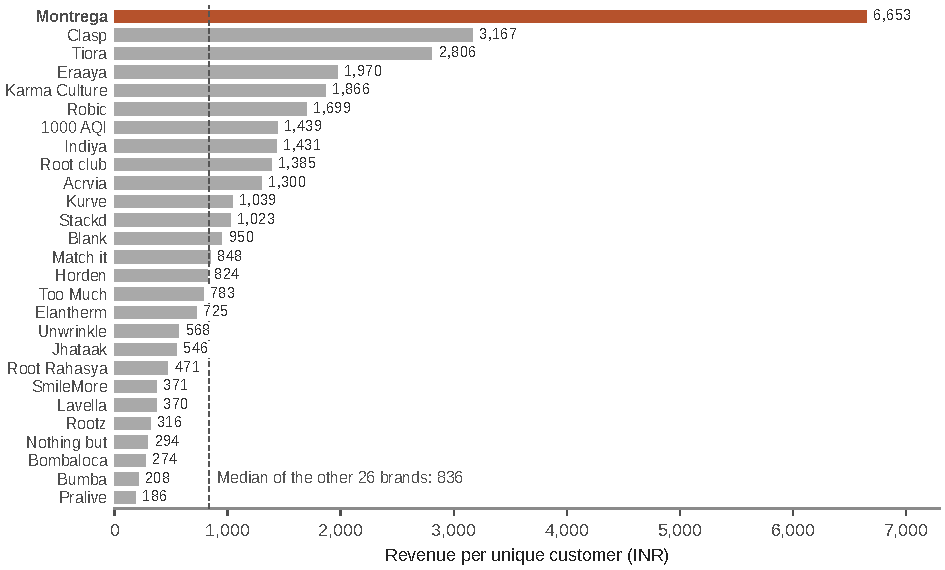
\includegraphics[width=\textwidth]{../figures/figure1.pdf}\par}
\fignote{\textit{Note:} The dashed line marks the median of the other 26 brands (\INR836); their mean is \INR1,033. \textit{Source:} TETR College of Business leaderboard, 22:00, 12 April 2026; author's calculations.}
\end{figure}

\section{Method}
Revenue is the product of three numbers: $R = C \times (U/C) \times (R/U)$, where $C$ is unique customers, $U$ units sold and $R/U$ the realized price per unit. In logs the product becomes a sum, $\ln R = \ln C + \ln(U/C) + \ln(R/U)$, so the variance of log revenue across brands splits into three covariances. For each part $x$ I report its share, $\mathrm{cov}(\ln x, \ln R)/\mathrm{var}(\ln R)$, which equals the slope from regressing $\ln x$ on $\ln R$. The three shares add to one. Trade economists use the same split to separate the margins along which countries export (Hummels and Klenow 2005; Bernard et al.\ 2009). Here customer count is the extensive margin, and units per customer and price per unit divide the intensive margin into quantity and price.

\section{Results}
Table~1 reports the shares. Across the 27 brands, price per unit carries 51 percent of the variance of log revenue, customer count 25 percent and units per customer 24 percent. Revenue and customer count have a Spearman rank correlation of 0.37 ($p = 0.06$). Twelve of the 26 other brands drew more customers than Montrega, and its 16 customers equaled their median (Figure~2).

\begin{figure}[H]
\figtitle{Figure 2. At 16 customers, brand revenue ranged from INR 22,895 to INR 106,450}{Revenue and unique customers by brand, log scales. Vasant Kunj market, 12 April 2026.}
{\centering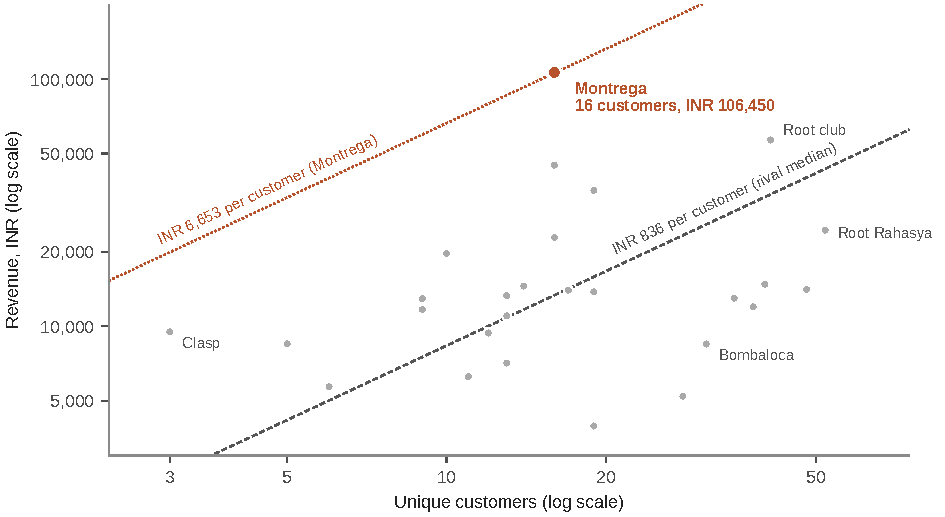
\includegraphics[width=\textwidth]{../figures/figure2.pdf}\par}
\fignote{\textit{Note:} Each straight line holds revenue per customer constant. Brands above the dashed line earned more per customer than the median of the other 26 brands. Spearman $\rho = 0.37$ ($p = 0.06$). \textit{Source:} as Figure~1.}
\end{figure}

Two checks qualify the result. Leaving out one brand at a time, price per unit keeps the largest share in all 27 runs (43 to 58 percent) and customer count stays between 19 and 36 percent. The basket share rests on Montrega: without it, units per customer carries 6 percent. A bootstrap over brands gives wide 90 percent intervals, 3 to 58 percent for customer count, so I treat the order of the three parts as better established than their size. At Galleria Market customer count carries 3 percent and price per unit more than all of the variance, because larger baskets went with lower revenue there.


\begin{table}[H]
\figtitle{Table 1. Price per unit carried the largest share of revenue differences}{Share of the cross-brand variance of log revenue, by component.}
{\centering\small
\begin{tabular}{@{}l>{\raggedleft\arraybackslash}p{1.55cm}>{\raggedleft\arraybackslash}p{1.75cm}>{\raggedleft\arraybackslash}p{1.6cm}>{\raggedleft\arraybackslash}p{2.75cm}@{}}
\toprule
 & Customers & Units per customer & Price per unit & Spearman $\rho$, revenue and customers \\
\midrule
Vasant Kunj, 27 brands & 25\% & 24\% & 51\% & 0.37 (0.06) \\
Vasant Kunj, without Montrega & 36\% & 6\% & 58\% & 0.40 (0.04) \\
Vasant Kunj, one brand left out & 19 to 36\% & 6 to 30\% & 43 to 58\% & \\
Galleria Market, 18 brands & 3\% & $-$11\% & 108\% & 0.05 (0.84) \\
\bottomrule
\end{tabular}\par}
\fignote{\textit{Note:} Each share is $\mathrm{cov}(\ln x, \ln R)/\mathrm{var}(\ln R)$; the three shares in a row add to 100 percent. The third row gives the range over 27 runs that each drop one brand. Bootstrap 90 percent intervals for the first row (10,000 resamples of brands): customers 3 to 58, units per customer $-$5 to 47, price per unit 20 to 83 percent. Two-sided $p$-values in parentheses, from the $t$ approximation. \textit{Source:} TETR College of Business leaderboards; author's calculations.}
\end{table}

\section{One brand at two markets}
Montrega ranked first at both markets (Table~2). Between Galleria and Vasant Kunj its customers fell from 31 to 16 while its bottles per customer rose from 1.52 to 6.13, a factor of 4.04. Its realized price per bottle fell from \INR1,678 to \INR1,086 (\x0.65), so revenue per customer rose 2.62 times ($4.04 \times 0.65$). With the rival median basket of 1.3 bottles and its own customers and price, Montrega would have earned about \INR22,500 and ranked sixth; that counterfactual ignores the link between basket size and price per bottle. The 15 rival brands that sold at both markets did not share the jump: their median basket changed by \x0.93, and only Indiya's rose by more than half (\x2.14).

\begin{table}[H]
\figtitle{Table 2. Montrega's basket quadrupled; the median matched rival's basket fell 7 percent}{Montrega at the two markets it won, with the 15 rival brands present at both.}
{\centering\small
\begin{tabular}{@{}l>{\raggedleft\arraybackslash}p{2.3cm}>{\raggedleft\arraybackslash}p{2.3cm}>{\raggedleft\arraybackslash}p{2.4cm}@{}}
\toprule
 & Galleria Market & Vasant Kunj & Vasant Kunj $\div$ Galleria \\
\midrule
Rank by revenue & 1st of 18 & 1st of 27 & \\
Unique customers & 31 & 16 & 0.52 \\
Units sold & 47 & 98 & 2.09 \\
Units per customer & 1.52 & 6.13 & 4.04 \\
Price per unit (INR) & 1,678 & 1,086 & 0.65 \\
Revenue per customer (INR) & 2,544 & 6,653 & 2.62 \\
Revenue (INR) & 78,850 & 106,450 & 1.35 \\
\midrule
15 matched rivals, median ratio: units per customer & & & 0.93 \\
15 matched rivals, median ratio: customers & & & 0.46 \\
\bottomrule
\end{tabular}\par}
\fignote{\textit{Note:} Units are bottles of 30\,ml or 100\,ml. Ratios use unrounded values. I matched rival brands by name across the two leaderboards. \textit{Source:} TETR College of Business leaderboards (Galleria Market, 21:00; Vasant Kunj, 22:00, 12 April 2026); author's calculations.}
\end{table}

\section{Three explanations for the basket}
\textit{(i) Quantity discounts.} We priced two-bottle bundles below two single bottles, a form of second-degree price discrimination: each buyer picks a quantity and with it a price per bottle. Bundles alone cannot produce the realized price. \INR1,086 per bottle sits below \INR1,100, the per-bottle price of our cheapest listed bundle (two 30\,ml bottles for \INR2,200), so at least \INR1,350 of the discounts at Vasant Kunj went beyond the price list.

\textit{(ii) A volume buyer buying gifts.} One customer bought more than ten bottles and asked for them to be gift-wrapped, and we recall one or two other wrapping requests that day.\footnote{From the stand team's recollection; no receipt records the order or the requests.} A negotiated price on that order could explain the discount gap: if every other bottle sold at the bundle price, twelve bottles at about \INR990 each would close it. The order cannot explain the basket. If it was 12 bottles, the other 15 customers averaged 5.7 bottles each, 3.8 times the Galleria basket; if it was 20, they averaged 5.2, still 3.4 times.

\textit{(iii) Audience and information.} Vasant Kunj shoppers may have bought more per head, or testing a fragrance on skin at the stand may have made a second or third bottle feel less risky. The 15 rival brands present at both markets argue against an effect on the whole market: their median basket changed by \x0.93, and 10 of the 15 fell. An effect limited to fragrance, where buyers judge the product only after wearing it, survives that check.

\section{What would separate them}
Three additions would do it: a receipt for every sale with product, quantity and discount; one question at the till about gifts; and a bundle offered in some hours or markets and withheld in others, across three or more markets. A regression of units per customer on a bundle indicator and a gift indicator, with stand position as a control, would then test (i) against (ii) and (iii). We recorded none of these, and stand position is missing from both markets.

\section{Limits and scope}
Sixteen customers at one event, counts kept by the organizer, one evening per market and no transaction-level data: the numbers describe these two markets and identify no cause. The note covers stand sales only. We ran no paid online advertising. We judged India's fragrance category too crowded with advertising for a new brand to stand out on a small budget, so we spent our money on testing formulations and used the stands TETR provided to confirm demand before paying for reach ourselves. The online store took five orders in the term, one of them a genuine sale; that record reflects a channel we never built and says little about demand. The test I would run is a small fixed advertising budget, with acquisition cost per customer measured against the average order and set beside the 30 percent or so of stand visitors who bought, a rate we counted at three events.

\section*{Appendix A: prices and data checks}
At Vasant Kunj a 30\,ml bottle listed at \INR1,300 and two 30\,ml bottles at \INR2,200. 100\,ml bottles sold for between \INR3,100 and 3,500, depending on the discount given at the stand; the point-of-sale export for Galleria Market shows averages of \INR3,375 to 3,500 by product. That export records 51 items and \INR80,300 against the leaderboard's 47 units and \INR78,850. Four extra bottles cannot add only \INR1,450 at listed prices, so the two systems did not count the same sales; I use the organizer's leaderboards throughout. Four brand names differ between the two leaderboards in capitalization or spelling (Jhataak and Jhatak, for example); I treat each pair as one brand.

\section*{References}
{\small
Bernard, Andrew B., J. Bradford Jensen, Stephen J. Redding, and Peter K. Schott. 2009. ``The Margins of US Trade.'' \textit{American Economic Review} 99 (2): 487--93.

Hummels, David, and Peter J. Klenow. 2005. ``The Variety and Quality of a Nation's Exports.'' \textit{American Economic Review} 95 (3): 704--23.\par}


\clearpage
\section*{Appendix B: source leaderboards}
The two leaderboards as the organizer published them. Every leaderboard figure in this note comes from these two images.

\vspace{6pt}
\noindent\begin{minipage}[t]{0.47\textwidth}
\centering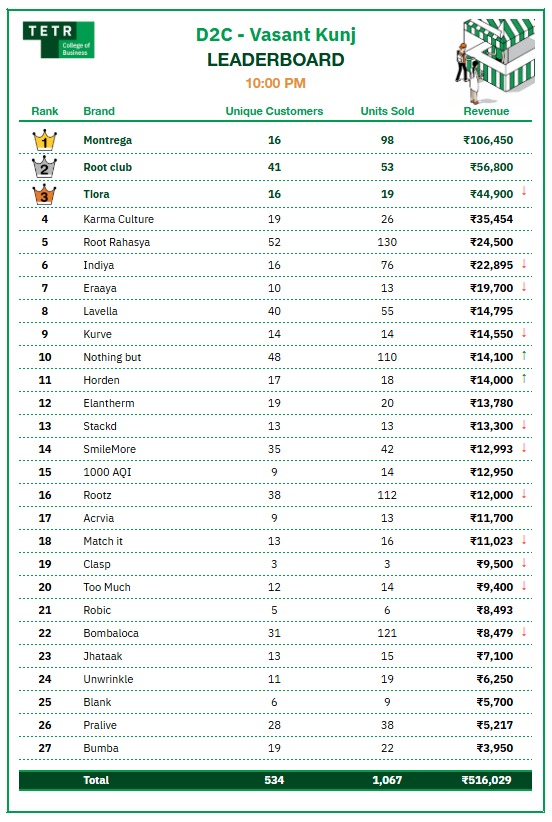
\includegraphics[width=\linewidth]{../data/source/vasant_kunj_leaderboard.jpeg}\\[3pt]
{\footnotesize Vasant Kunj, 22:00, 12 April 2026 (27 brands).}
\end{minipage}\hfill
\begin{minipage}[t]{0.47\textwidth}
\centering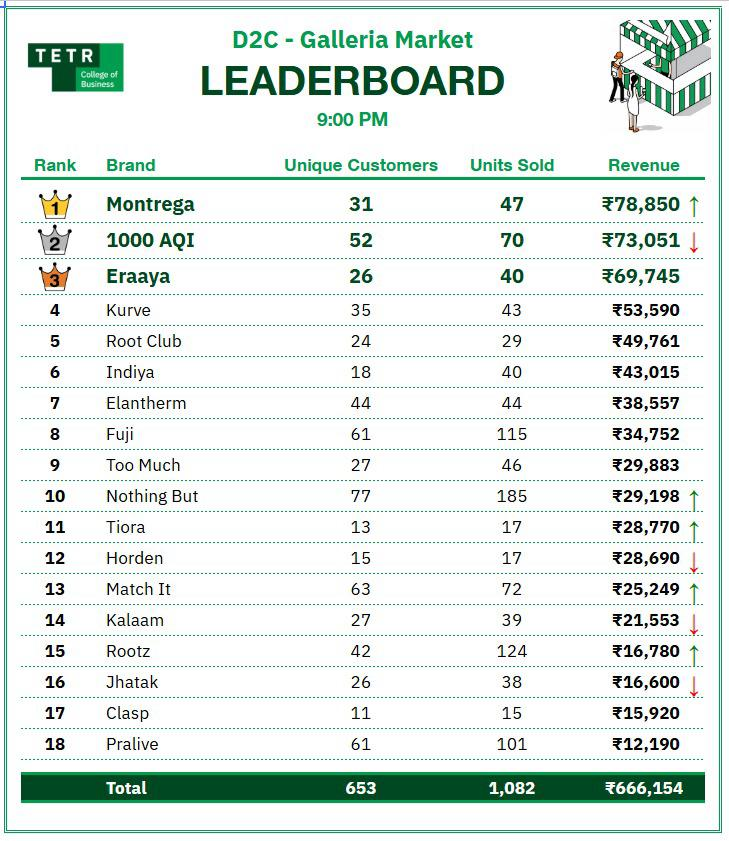
\includegraphics[width=\linewidth]{../data/source/galleria_market_leaderboard.jpeg}\\[3pt]
{\footnotesize Galleria Market, 21:00, date not printed (18 brands).}
\end{minipage}

\vspace{8pt}
{\footnotesize \textit{Source:} TETR College of Business.}

\end{document}
